\documentclass[11pt]{article}
\usepackage[a4paper,top=0.6cm,bottom=3.0cm,left=1.9cm,right=1.9cm,footskip=2.0cm]{geometry}
\usepackage{graphicx}
\usepackage[table]{xcolor}
\usepackage{ragged2e}
\usepackage{fancyhdr}
\usepackage{fontspec}
\setmainfont{Carlito}
\setsansfont{Carlito}
\newfontfamily\latinfont{Carlito}
\renewcommand{\familydefault}{\sfdefault}
\definecolor{titleblue}{HTML}{0F2F4A}
\definecolor{textblack}{HTML}{1A1A1A}
\definecolor{rule}{HTML}{C9C4C0}
\definecolor{muted}{HTML}{6B635E}
\setlength{\parindent}{0pt}\setlength{\parskip}{0.5em}

\setlength{\headheight}{28pt}\setlength{\headsep}{6pt}
\newcommand{\idmfooter}{%
  \begin{minipage}{\textwidth}
    {\color{rule}\hrule height 0.7pt}\vspace{4pt}
    \noindent
    \begin{minipage}[c]{0.66\textwidth}{\scriptsize\color{muted}Developed by the Water and Climate Lab, IIT Gandhinagar, using hydro-meteorological data from partner agencies.}\end{minipage}\hfill
    \begin{minipage}[c]{0.32\textwidth}\raggedleft
      
\includegraphics[height=0.62cm]{wcl.png}\hspace{6pt}%
      
\includegraphics[height=0.62cm]{iitgn.png}
    \end{minipage}\\[3pt]
    {\scriptsize\color{muted}© 2026 Water and Climate Lab · Indian Institute of Technology Gandhinagar · For research and demonstration purposes.}
  \end{minipage}%
}
\newcommand{\idmrunhead}{%
  \begin{minipage}{\textwidth}
    {\small\bfseries\color{titleblue}National Drought Summary}\hfill{\small\color{muted}Week ending May 20, 2026}\\[2pt]
    {\color{rule}\hrule height 0.6pt}
  \end{minipage}%
}
\fancypagestyle{idmfoot}{\fancyhf{}\renewcommand{\headrulewidth}{0pt}\renewcommand{\footrulewidth}{0pt}\fancyfoot[C]{\idmfooter}}
\fancypagestyle{idmrun}{\fancyhf{}\renewcommand{\headrulewidth}{0pt}\renewcommand{\footrulewidth}{0pt}\fancyhead[C]{\idmrunhead}\fancyfoot[C]{\idmfooter}}
\pagestyle{idmrun}

\begin{document}

\thispagestyle{idmfoot}
\noindent
\begin{minipage}[c]{0.16\textwidth}
\includegraphics[width=\linewidth]{wcl.png}\end{minipage}\hfill
\begin{minipage}[c]{0.80\textwidth}\raggedleft
  {\fontsize{19}{22}\selectfont\bfseries\color{titleblue}National Drought Summary}\\[2pt]
  {\normalsize\color{muted}Week ending May 20, 2026}
\end{minipage}
\vspace{6pt}{\color{rule}\hrule height 1pt}\vspace{10pt}
\begin{center}
  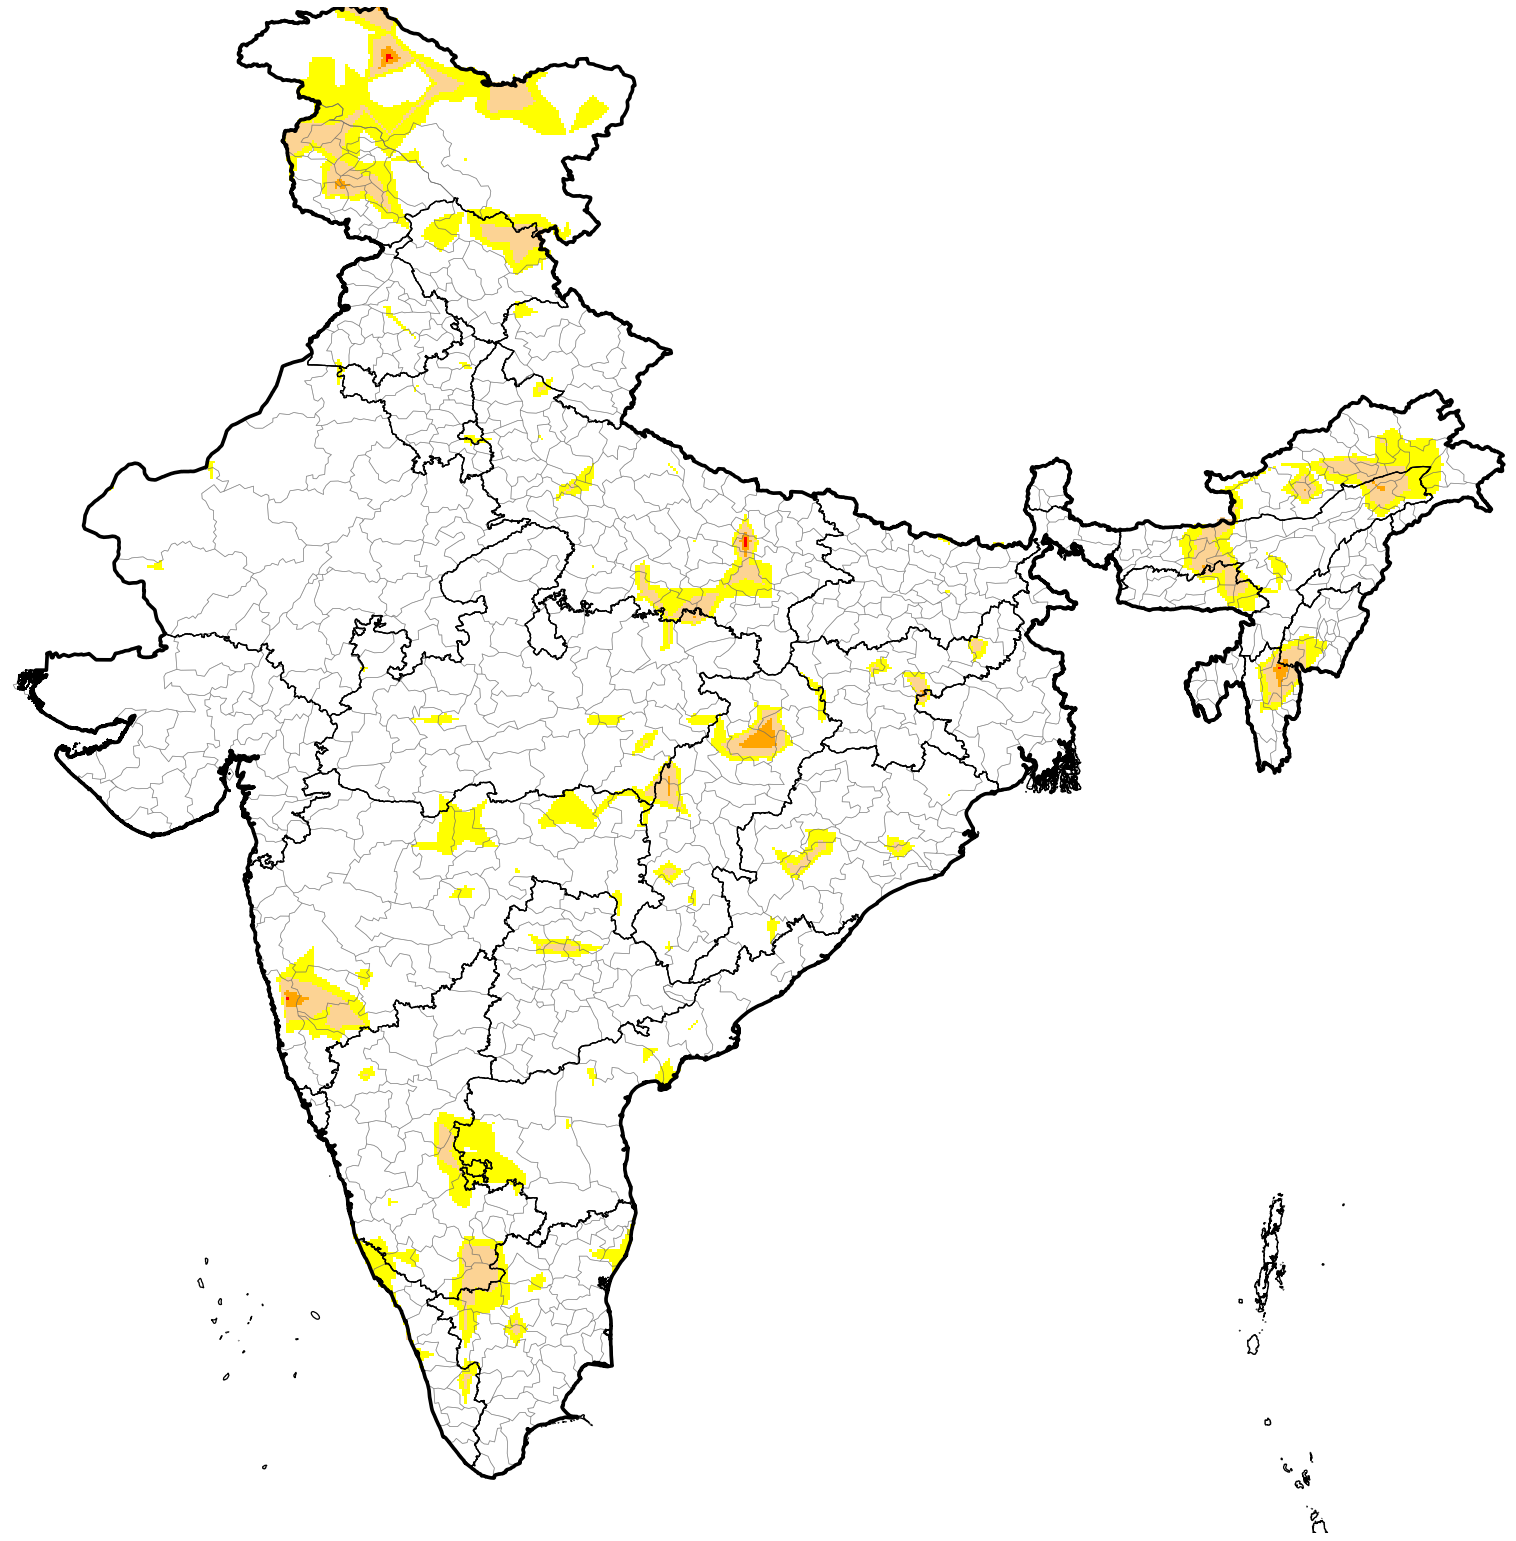
\includegraphics[width=0.60\textwidth]{cdi_map.png}\\[3pt]
  {\small\color{muted}Combined Drought Index (CDI) for the week ending May 20, 2026.}
\end{center}
\vspace{2pt}
{\large\bfseries\color{titleblue}Summary}\\[3pt]
{\justifying\normalsize\color{textblack}The national drought situation this week shows a majority of the area in the Normal category, with a small portion experiencing drought conditions. The total area experiencing drought, classified as D0 or worse, was 15.3\% this week. This figure reflects a contraction in the drought area compared to the previous week, which was 16.2\%, indicating a decrease of 0.9 percentage points week-on-week. The most affected regions by drought were NCT of Delhi, Manipur, Mizoram, Arunanchal Pradesh, Jammu \& Kashmir, and Meghalaya. Conversely, West Bengal reported 0.0\% of its area in drought, while Rajasthan, Gujarat, and Telangana reported 1.0\%, 2.1\%, and 3.4\% of their areas in drought, respectively.\par}
\vspace{8pt}
{\large\bfseries\color{titleblue}Regional Outlook}\\[2pt]
{\normalsize\color{titleblue}\textbf{North}}\enspace {\normalsize\color{textblack}Moderate, scattered drought. About 28\% of the area is in drought (D0–D4).} \par\smallskip {\normalsize\color{titleblue}\textbf{Northwest}}\enspace {\normalsize\color{textblack}Largely normal conditions. About 4\% of the area is in drought (D0–D4).} \par\smallskip {\normalsize\color{titleblue}\textbf{Northeast}}\enspace {\normalsize\color{textblack}Moderate, scattered drought. About 27\% of the area is in drought (D0–D4). Pockets of severe-or-worse conditions are present.} \par\smallskip {\normalsize\color{titleblue}\textbf{East}}\enspace {\normalsize\color{textblack}Mostly normal, with localised dryness. About 7\% of the area is in drought (D0–D4).} \par\smallskip {\normalsize\color{titleblue}\textbf{Central}}\enspace {\normalsize\color{textblack}Mostly normal, with localised dryness. About 15\% of the area is in drought (D0–D4). Pockets of severe-or-worse conditions are present.} \par\smallskip {\normalsize\color{titleblue}\textbf{West}}\enspace {\normalsize\color{textblack}Moderate, scattered drought. About 22\% of the area is in drought (D0–D4).} \par\smallskip {\normalsize\color{titleblue}\textbf{South}}\enspace {\normalsize\color{textblack}Mostly normal, with localised dryness. About 16\% of the area is in drought (D0–D4).}
\end{document}
